\chapter{Lattice Examples}
\label{c:lat.example}

This chapter gives some examples of how lattice files can be constructed to
describe various machine geometries.

%-----------------------------------------------------------------------------
\section{Example: Injection Line}
\label{s:ex.inj}

\begin{figure}[tb]
  \centering
  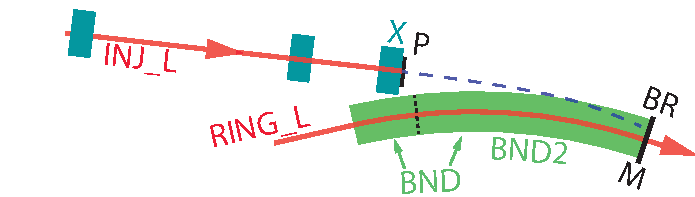
\includegraphics[width=5in]{injection.pdf}
  \caption[Injection line into a dipole magnet.]{
Injection line into a dipole magnet.
  }
  \label{f:inject}
\end{figure}

An injection line is illustrated in \fig{f:inject}. In this example,
The path of an injected particle after it leaves the last element
\vn{X} of the injection line (dashed blue line) partially goes through
the field of the dipole \vn{BND} in the storage ring. One way to
simulate this is:
\begin{example}
  INJ_L: line = (..., X, P, BND2, BR)
  RING_L: line = (..., BND, M, ...)
  P: patch, x_offset = -0.5, x_pitch = 0.15, z_offset = 0.3 
  BND: sbend, l = 6.2, g = 1/52
  BND2: BND, l = 4.7, tracking_method = runge_kutta,
          field_calc = grid, field = \{...\}
  BR: fork, to_line = RING_L, to_element = M
  M: marker
  use, INJ_L
\end{example}

In order to properly track particles through the fringe field of the
dipole \vn{BND}, a partial section of \vn{BND}, called \vn{BND2}, is
placed in the injection line \vn{INJ_L}. The \vn{tracking_method} for
\vn{BND2} is set to \vn{runge_kutta} since the default
\vn{bmad_standard} tracking is not able to handle these fringe
fields. Additionally, the \vn{field_calc} parameter of \vn{BND2} is
set to \vn{grid} so that the actual field profile of this particular
magnet can be used in the tracking. The field is specified in the
\vn{field} parameter (\sref{s:em.fields}). 

After traversing element \vn{X} in the injection line, the particle
goes through the patch \vn{P} which offsets the reference trajectory
so that following element, \vn{BND2}, is properly positioned.  The
beginning of \vn{BND2} is marked by a black dashed line in the figure.
At the end of \vn{BND2} the fork element \vn{BR} connects \vn{INJ_L}
with the marker \vn{M} in \vn{RING_L}.

%-----------------------------------------------------------------------------
\section{Example: Energy Recovery Linac}
\label{s:ex.erl}

\begin{figure}[tb]
  \centering
  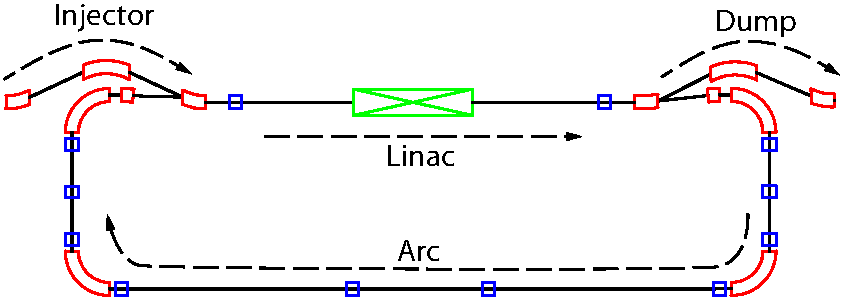
\includegraphics[width=6in]{erl.pdf}
  \caption[Example Energy Recovery Linac.]{
Example Energy Recovery Linac. A) The ERL consists of an injection
line, accelerating linac, return arc, decellerating linac, and finally
a beam dump. B) Close up of the section where the end of the injector
and the end of the arc inject into the beginning of the linac. C)
Close up of the end of the linac which injects into the dump and the
beginning of the arc.}
  \label{f:erl}
\end{figure}

An Energy Recovery Linac (ERL) is illustrated in \fig{f:erl}A. The ERL
starts with an injection line that feeds a linac which accelerates the
beam to some energy. The beam then transverses a return \vn{arc} which
reinjects the bunches into the linac. The length of the return arc is
such that, on the second pass, the beam is decelleratied giving its
energy back to the RF cavities. Finally, the decelleratied beam is
steered through a dump line where, at the end, an absorber stops the
beam.

 A lattice file for modeling this ERL:
\begin{example}
  parameter[geometry] = open
  parameter[absolute_time_tracking] = T

  BEND_L1: sbend, angle = -25*pi/180, l = 0.2, ...
  BEND_L2: BEND_L1

  A_PATCH: patch, flexible = T
  D_PATCH: patch, x_offset = 0.034, x_ptich = asin(0.32) 
  INJECT: line = (...)
  LINAC: line[multipass] = (BEND_L1, ..., BEND_L2)
  ARC: line = (..., BEND_A7)
  DUMP: line = (...)

  ERL: line = (INJECT, LINAC, ARC, A_PATCH, LINAC, D_PATCH, DUMP)
\end{example}

\index{patch!example}
\fig{f:erl}B shows the injector and arc merging into the beginning of
the linac. The first element of the linac is a bend named
\vn{BEND_L1}. The bending angle for \vn{BEND_L1} has been set at the
appropriate value for injection from the injector. To get the correct
geometry for injection from the arc, a \vn{patch} element, named
\vn{A_PATCH}, is placed in the \vn{ERL} line between the arc and the
linac. \vn{A_PATCH} is a flexible patch which means that the exit edge
of \vn{A_PATCH} will automatically be aligned with the entrance edge
of the next element which is \vn{BEND_L1}. 

Note that this use of a flexible patch works since the orientation of
\vn{BEND_L1} has been determined before the orientaiton of
\vn{A_PATCH} is determined. The orientaiton of elements is determined
in order starting from the first element in the line (the exception to
this rule is if there is a \vn{floor_position} element) and the
orientation of \vn{BEND_L1} is thus determined right after the
injector section on the first pass through the linac.



\fig{f:erl}C shows the end of the linac splitting off into the dump
and arc sections. The l

A patch
element named \vn{A_PATCH} is used

%-----------------------------------------------------------------------------
\section{Example: Patch Between reversed and non-reversed elements}
\label{s:ex.patch}

\begin{figure}[tb]
  \centering
  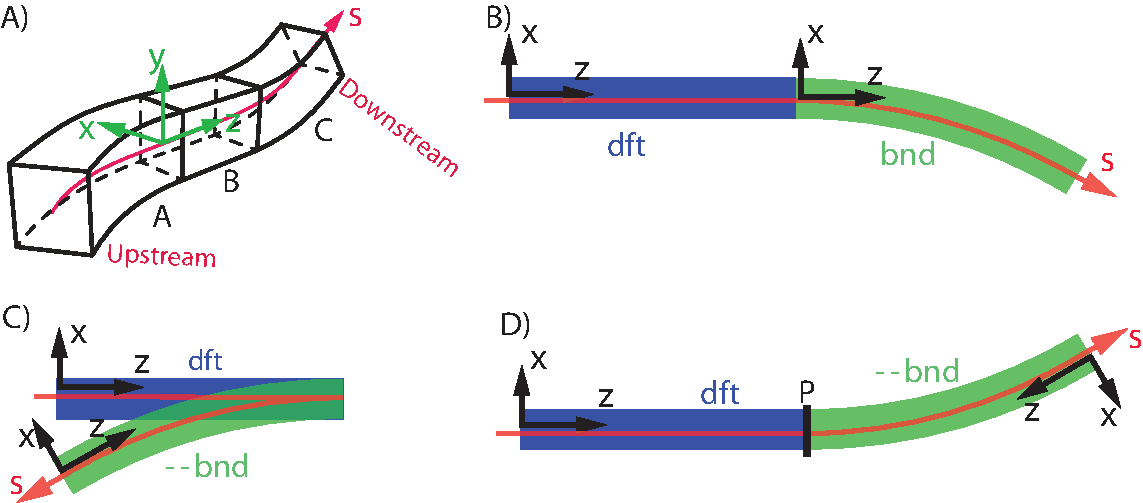
\includegraphics[width=5in]{patch-between.pdf}
  \caption[Patching between reversed and non-reversed elements.]{
Drift element \vn{D} is followed by a reversed drift element \vn{B}.
The view is from $+y$ onto the $x$-$z$ plane. A) If no patch is
present then the geometry does not make physical sense. B) With a
patch in between, a sane geometry can be obtained.}
  \label{f:patch.between}
\end{figure}

\index{patch}
Between normal and reversed elements there must be a reflection
\vn{patch} element (\sref{s:patch}).  This is illustrated in
\fig{f:patch.between}. The basic lattice is
\begin{example}
  D: drift, l = 2
  g_design = pi/12
  B: sbend, l = 2, g = g_design, g_err = -2*g_design
  P: patch, x_pitch = pi
  A_line: line = (D, --B)     ! Illegal. Do not use!
  B_line: line = (D, P, --B)  ! Correct
\end{example}
Line \vn{A_line} represents the situation shown in
\fig{f:patch.between}A.  With no patch between the drift \vn{D} and
the reversed bend \vn{B}, a particle leaving \vn{D} at \vn{D}'s
downstream end will find itself outside of both \vn{D} and
\vn{B}. Clearly this is an unphysical situation. Sanity is restored in
line \vn{B_line} shown in \fig{f:patch.between}B. In this instance, the
patch \vn{P} rotates the reference coordinates around the $y$-axis
leaving the $y$-axis invariant the bend of \vn{B} is in the $x$-$z$
plane. There are other patch parameter values that could be used to
produce a reflection patch (\sref{s:reflect.patch}).  For example,
Setting the patch's \vn{y_pitch} to \vn{pi} would produce a reflection
patch.

Since bend \vn{B} is reversed, A particle moving downstream within
\vn{B} is going the opposite direction from the normal direction. If
\vn{g_err} were zero in this instance, a downstream moving particle
would feel a force that will rotate the particle in a clockwise manner
opposite from the counterclockwise direction of the bend. To counter
this, \vn{g_err} is set so the total bending field \vn{g_tot = g +
g_err} is opposite the design field. That is, \vn{g_err} is set so
that \vn{g_tot = -g}.

%-----------------------------------------------------------------------------
\section{Example: Colliding Beam Storage Rings}
\label{s:ex.collide}

\begin{figure}[tb]
  \centering
  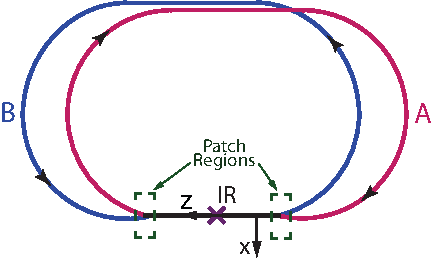
\includegraphics[width=5in]{colliding-beams.pdf}
  \caption[Dual ring colliding beam machine]{Dual ring colliding beam machine. 
The beam in the \vn{A} ring rotates clockwise and in the \vn{B} ring
counterclockwise.}
  \label{f:collide}
\end{figure}

The idealized layout of a pair of storage rings used for colliding
counter rotating beams is shown in \fig{f:collide}. Rings \vn{A} and
\vn{B} intersect at two interaction regions labeled \vn{ir1} and
\vn{ir2} where the beams collide. The basic lattice description is:
\begin{example}
  ir1: line[multipass] = (...)
  ir2: line[multipass] = (...)
  pa1_in; patch, ...
  pa1_out; patch, ...
  pa2_in; patch, ...
  pa2_out; patch, ...
  m: marker
  fid: fiducial, origin_ele = m
  ...
  A: line = (arc_a1, pa1_in, ir1, m, pa1_out, arc_a2, pa2_in, ir2, pa2_out)
  B_rev: line = (arc_b1, pb1_in, ir1, fid, pb1_out, arc_b2, pb2_in, ir2, pb2_out)
  B: line = (--B_rev)
  use, A, B
\end{example}
Lines \vn{ir1} and \vn{ir2} are the two interaction regions which are
declared \vn{multipass} since they are shared by the two rings. Line
\vn{A} represents ring \vn{A} where the beam which, by definition,
travels in the same direction as increasing $s$, rotates clockwise.
Line \vn{B_rev} is a ``reversed'' line of ring \vn{B} and, like
\vn{a}, represents a beam rotating clockwise.  Line \vn{B}, which
represents ring \vn{B}, is the reverse of \vn{B_rev} and here the beam
rotates counterclockwise. In this construction, all elements of \vn{B}
are reversed.  While this is not mandatory (only the interaction
regions must be reversed in \vn{B}), having all of \vn{B} reversed
simplifies the geometry since this Means that the local coordinate
systems of both lines \vn{A} and \vn{b} will be ``aligned'' with the
$x$-axis pointing to the outside of the ring and the $y$-axis pointing
up, out of the page. Having non-aligned coordinate systems is possible
but potentially very confusing.

The two rings are physically aligned using a marker \vn{m} in \vn{A}
and a \vn{fiducial} element \vn{fid} in \vn{B} that aligns with
\vn{m}.  Each ring has four rigid \vn{patch} elements, whose name
begins with \vn{p}, on either side of each interaction region.

The finished lattice will have two branches, The first branch (with
index 0) will be derived from line \vn{a} (and hence will be named
``a'') and the second branch (with index 1) will be derived from line
\vn{b} (and hence will be named ``b''). The multipass lords
representing the physical IR elements will be in the ``lord section''
of branch 0.
